\documentclass[twocolumn,9pt]{extarticle}
\usepackage[hmargin=2cm,vmargin=2cm]{geometry}
\setlength{\columnsep}{18pt}
\usepackage{setspace}
\usepackage{graphicx}
\usepackage{caption}
\usepackage{algorithm}
\usepackage{algpseudocode}
\usepackage{amsmath}
\usepackage{subfigure}
\usepackage{times,parskip}
\usepackage{cleveref}
\usepackage{listings}
\graphicspath{ {images/} }
\begin{document}
\title{\textbf{A Simple Review About Maximum Flow Problem}}
\author{Xiao Liang \thanks{3130103863} \and Jie Li \thanks{3130103725} \and Yicun Zheng \thanks{3130104113}}
\date{\today}
\maketitle

\begin{abstract}
In this review, we first describe the meaning of maximum flow problem, then make some explanations of some famous algorithms on this problem which include augmenting path algorithm (Ford-Fulkerson Algorithm), shortest augmenting path algorithm (Edmonds-Karp Algorithm), blocking flow algorithm (Dinic's Algorithm), push and rebalel algorithm (Goldberg and Tarjan). And we introduce the dynamic tree, which is very useful in reducing time complexity of maximum flow problem. Finally, we make some explanations of the test result of these algorithms we implemented.
\end{abstract}


\section{Introduction Of Maximum Flow Problem}
For a given graph $G(V,E)$, every edge has a capacity, which represents the max quantity of flow can flow over it. There are two special points in graph G, source and target, source can outflow infinite mount of flow and target can absorb infinite mount of flow. Every edge in the graph is directed, which means the flow in one edge can only has one direction. It's quite resonable, because we can always cancel out the encounter part of flows in one edge. Every point cannot store flow, which means the mount of flow flows into a certain point is equal to the mount of flow flows out of the point. And the question is, what's the maximum of flow which can flows from source to target.
If we use $c(e)$ to represent the capacity of edge $e$, $f(e)$ to represent the mount of flow in edge $e$, the request is:
\begin{equation}
	\begin{cases}
		0 \leq f(e) \leq c(e) \quad e \in E \\
		\sum_{e\ into\ v}{f(e)} = \sum_{e\ out\ of\ v}{f(e)} \quad v \in V-\{s,t\}
	\end{cases},
\end{equation}
and the target is:
\begin{equation}
\max_{e\ into\ t}{f(e)}.
\end{equation}

\section{Augmenting Path Algorithm}
For maximum flow problem, one basic idea is greedy method, which select one path $P=(v_1, v_2, ..., v_k)\ where\ k\geq\ 2,\ v_1=s,\ v_k=t$ from source to target each time, and add the flow as much as possible, cut down the quantity of flow from corresponding capacities along the path. However, greedy method cannot make sure to get the optimal result, just like greedy method cannot get the optimal result in many other problems. When we choose one path, it's not possible to cancel it in greedy method. In order to make it possible, this algorithm uses "Residual Path" to point out a special path which has opposite direction of the flow flows a certain edge and the same mount of quantity. Imagine that, if next path flows along a residual path, it means that the original flows flow over this edge are reduced, which has the effect of adjusting the flows over a certain edge, and this is exactly what we want. In this algorithm, every path from source to target is named as "Augmenting Path", and we get the maximum flow by find out all augmenting path in the graph. Everytime we find an augmenting path, we need to add corresponding residual path to the graph. In order to finish the algorithm as fast as possible, everytime we find an augmenting path, we need to add as much flow as possible, which means that we need to find minimum capacity along the path and use it as the quantity of flows along the path.

It's possible that everytime we can only add one quantity of flow into the maximum flow, which can be fulfilled by a carefully constructed graph; therefore, if the maximum flow is $F$, we need $F$ augmenting paths to get the maximum flow. By using Dijkstra algorithm to find an augmenting path, the time complexity of finding one augmenting path is $O(VE)$, and the total time complexity of this algorithm is $O(VEF)$.

\section{Shortest Augmenting Path Algorithm}
The algorithm above can make sure to get the maximum flow. However, the time complexity in worst case is related to the quantity of maximum flow, which is not very good, because the maximum flow of a certain graph is unrelated to the scale of the graph, which means that even for a small graph, this algorithm may need a long time to solve it.

In order to make the time complexity unrelated to the quantity of maximum flow, Jack Edmonds and Richard Karp added the concept of "distance" into the flow graph, which is really an ingenious idea. The idea is, by assuming every edge has the distance of 1, we can calculate the distance from a certain point to source, and the distance from source and target in a certain path.

This algorithm finding the shortest augmenting path repeatedly by using breadth first search. And in every augmenting path, we use the same idea in section 1 to find the max quantity of flow that can flow over it.
Everytime we find an augmenting path, if edge $(u, v)$ is the edge with least capacity along the path, this edge will be saturated. And after saturating this edge, there will be a residual path over it with opposite direction. If we want to use this edge again, we need to find a path whose distance between $(s, u)$ along the path is larger than the distance between $(s, v)$ along the path. And after saturating it again, the condition becomes the distance between $(s, v)$ larger than $(s, u)$ again. The longest path in this graph can be $E$, so a certain edge can be saturated $V$ times at most, which means we can have $VE$ augmenting paths at most. The time complexity of finding an augmenting path by using breath first search is $O(E)$, so the time complexity of this algorithm is $O(VE^2)$.

\section{Blocking Flow Algorithm}
This algorithm is created by Yefim Dinic. This algorithm is similar to Shortest Augmenting Path Algorithm, but it uses breadth first scan to build the layer graph first, which can add more aumenting paths in one step rather than one path in Shortest Augmenting Path Algorithm. Therefore, the time complexity of this algorithm is $O(V^2E)$.

In this algorithm, we first use breadth first scan to search the path from source to target. When we find one path, we continue the scan in this layer, so we can get all shortest path from source to target. Then we use this layer graph to find flows from source to target, for every augmenting path, we don't need to add the residual path to the layer graph for now. When finding all augmenting path in this layer graph, we add the residual paths in this stage to the original flow graph, and use breadth first scan to find the shortest path in the new flow graph.

In every layer graph, we only use depth first scan algorithm to find usable flow path without adding residual path to the layer graph, so we may have a question: how can we make sure we can find all augmenting path with length k in kth layer graph? In fact, if we add the residual path into the kth layer graph, the augmenting path we find may be longer than k, which is conflict with the idea of this algorithm. And because we add residual paths after we scan every layer graph, so the flows we don't add in kth layer will has a longer length in residual graph and will be added to augmenting path in the layer graph later.

The longest path in flow grpha is $V$, so there are $V$ layer graph at most. For every layer graph we need $O(VE)$ to find the blocking flow. So the time complexity of this algorithm is $O(V^2E)$

Compared with Shortest Augmenting Path Algorithm which has time complexity of $O(VE^2)$, Blocking Flow Algorithm runs fast in dense graph.

\section{Push And Relabel Algorithm}
The push and relabel algorithm is created by A.V.Goldberg and R.E.Tarjan by manipulating the preflow in graph.
This algorithm is essentially different from the augmenting path algorithm described above. Push and relabel algorithm first preflows flows to saturate all nodes adjacent to source and manipulate excess flow (the flow still in node) between individual nodes.

The "label" in this algorithm is a non-negative integer of each node. We use $l(v)$ to represent the label of node $v$. At beginning, it makes $l(s)=n$ and $l(v)=0,\ v\ \in\ V-\{s\}$. Then it pushed as much flow as possible from $s$ to the adjacent node of $s$, so all path start with $s$ will be saturated. This process is called "preflow". After preflow, the algorithm begins to push and relabel. A relabel on a node increatese its label by at least one. If $l(u) > l(v)$, node $u$ and push flows to node $v$. The label of source and target will always be $n$ and $0$, which is very important to make sure the algorithm can finally stop.

One node can be relabelled if and only if this node has some excess, and the excess can be sent to nowhere. By this method, we can send flows backward, so if the actually maximum flow is smaller than preflow, the excess part of flow can finally be sent back to source, leaving the actual maximum flow.

In the beginning, all nodes except source has $l(v)=0$, so we keep relabel nodes to make sure the excess flow has path to go. At some stage, some nodes will be relabelled above $n$, at that moment, these nodes will have no excess (relabeling the node can make sure all excess flows out) and no other flows can reach them (the source only has label of $n$). So these nodes will become unreachable. And when all excess has been pushed to either source or target, the flows in the flow graph comes to stable, and the valid flow in the graph is just the maximum flow of the graph.

The pseudocode of push and relabel are shown as below:
\begin{algorithm}
\caption{Push precedure}
	\begin{algorithmic}[1]
		\Require: $v$ is active, $r(v,w)\ >\ 0$ and $l(v)=l(w)+1$
		PUSH(Edge($v$,$w$)):\\
			Transfer $\sigma=\min(e(v),r(v,w))$ units of flow by updating the edges $(v,w)$ and $(w,v)$, and the excess $e(v)$ and $e(w)$.\\
		END
	\end{algorithmic}
\end{algorithm}

\begin{algorithm}
\caption{Relabel procedure}
	\begin{algorithmic}[1]
		\Require: $v$ is active, $\forall w \in V,\ r(v,w) > 0,\ l(v) \le l(w)$
		RELABEL($v$):\\
		$l(v) = \min(l(w)+1 | (v,w) \in E, r(v,w)>0)$\\
		END
	\end{algorithmic}
\end{algorithm}

When a node have path to push its excess, we can use push procedure to push its excess to other nodes. The amount of flow can be pushed is limited by the residual capacity and the current label of that node. The excess of a node can never become negative, and the capacity constraint of path can never be violated. Sometimes, one node has excess left but has no way to push them, then we can use relabel procedure to relabel this node so as to make sure we can push the excess out of this node. This procedure keeps continuing until the excess of all nodes except target and source are zero. We can use a list to maintain the nodes whose excess is not zero, in every push procedure, at most one node can be removed from this list, and some node will be added to this list; in every relabel procedure, one node will be relabelled higher label and have chance to push its excess. When the list becomes empty, all nodes have no excess and the algorithm finishes.

This algorithm is very similar to push water from source and count the output speed of water at target. It's like a 
simulation of real physical phenomenon of maximum flow. So we think this algorithm may be more elegent, with time complexity of $O(V^3)$.

\section{More Recent Work}

\subsection{V.King and S.Rao's Algorithm}
This algorithm is a kind of push and relabel algorithm, which uses a game to simulate the algorithm's behavior. The game's purpose is to select edges, which determines which edge to push when pushing excess from a node. That is, V.King and S.Rao's algorithm improves push and relabel algorithm by make a better choice in push operation, which reduce the time complexity from $O(V^3)$ to $O(VE+V^{2+\epsilon})$ for any $\epsilon > 0$.

\subsection{A.V.Goldbery and S.Rao's Algorithm}
This algorithm is based on the idea of blocking flow. And it uses a binary length function to represent the length of edge, which means the length of every edge can be $0$ or $1$. The edges with large capacity are assigned with $0$ length and edges with small capacity are assigned with $1$ legnth. The main idea of this algorithm is to saturate the large eldges first by including them in an earlier layer graph. The time complexity of this algorithm is $O(\min\{V^\frac{2}{3},\sqrt{E}\}E\log(\frac{V^2}{E})\log{F})$.

\section{Dynamic Tree}
Dynamic tree is a kind of data structure presented by D.D.Sleator and R.E.Tarjan. Update operation of this data structure can be done in $O(\log{n})$ time, where $n$ is the size of the tree. Dynamic tree supports following operations:
\begin{itemize}
\item Link($a$,$b$): Let $b$ be a child of $a$, and $a$ need to be a root to make sure this link is reasonable.
\item Cut($a$): Remove $a$ from the tree where $a$ belongs to, and make $a$ become a root of a new tree.
\item SetCost($a$, $c$): Set the cost of $a$ to $c$.
\item GetCost($a$): Get the cost of $a$.
\item AddCost($a$,$c$): Add the cost of $a$ by $c$.
\item GetPathLength($a$): Get the length of path from the root of tree where $a$ belongs to to $a$.
\item GetRoot($a$): Get the root of tree where $a$ belongs to.
\item GetChildren($a$): Get the children of $a$.
\item GetMinCostNode($a$): Get the last node on path from a to the root of the tree $a$ belongs to which has the minimum capacity along the path.
\item GetBoundingNode($a$,$c$): Get the first node on the path from a th the root of the tree $a$ belongs to which has a cost less than or equal to $c$.
\end{itemize}
The dynamic tree is used to represent the graph structure in maximum flow problem. As for every update operation has $log(n)$ cost, the path finding operation in the algorithm above can be reduced from $O(n)$ to $O(\log(n))$.


\section{Implementation And Test Result}
In order to test the result of different maximum flow algorithm, we implemented three kind of them, where are Shortest Augmenting Path Algorithm, Blocking Flow Algorithm and Push and Relabel Algorithm. The source code of these algorithm is in the attachment.

We write a simple program to generate a random adjancent matrix as the input to test these algorithms. First you input a number $n$, then this program will generate $n\times n$ random numbers ranging from 0 and predefined max capacity. Considering that the adjancent matrix generated by random is quite dense, so this will lead bad performance for the shortest augmenting path algorithm, because shortest augmenting path algorithm takes $O(VE^2)$ and in a dense graph $E\sim V^2$.

And the test result for the Shortest Augmenting Path Algorithm, Blocking Flow Algorithm and Push and Relabel Algorithm is:
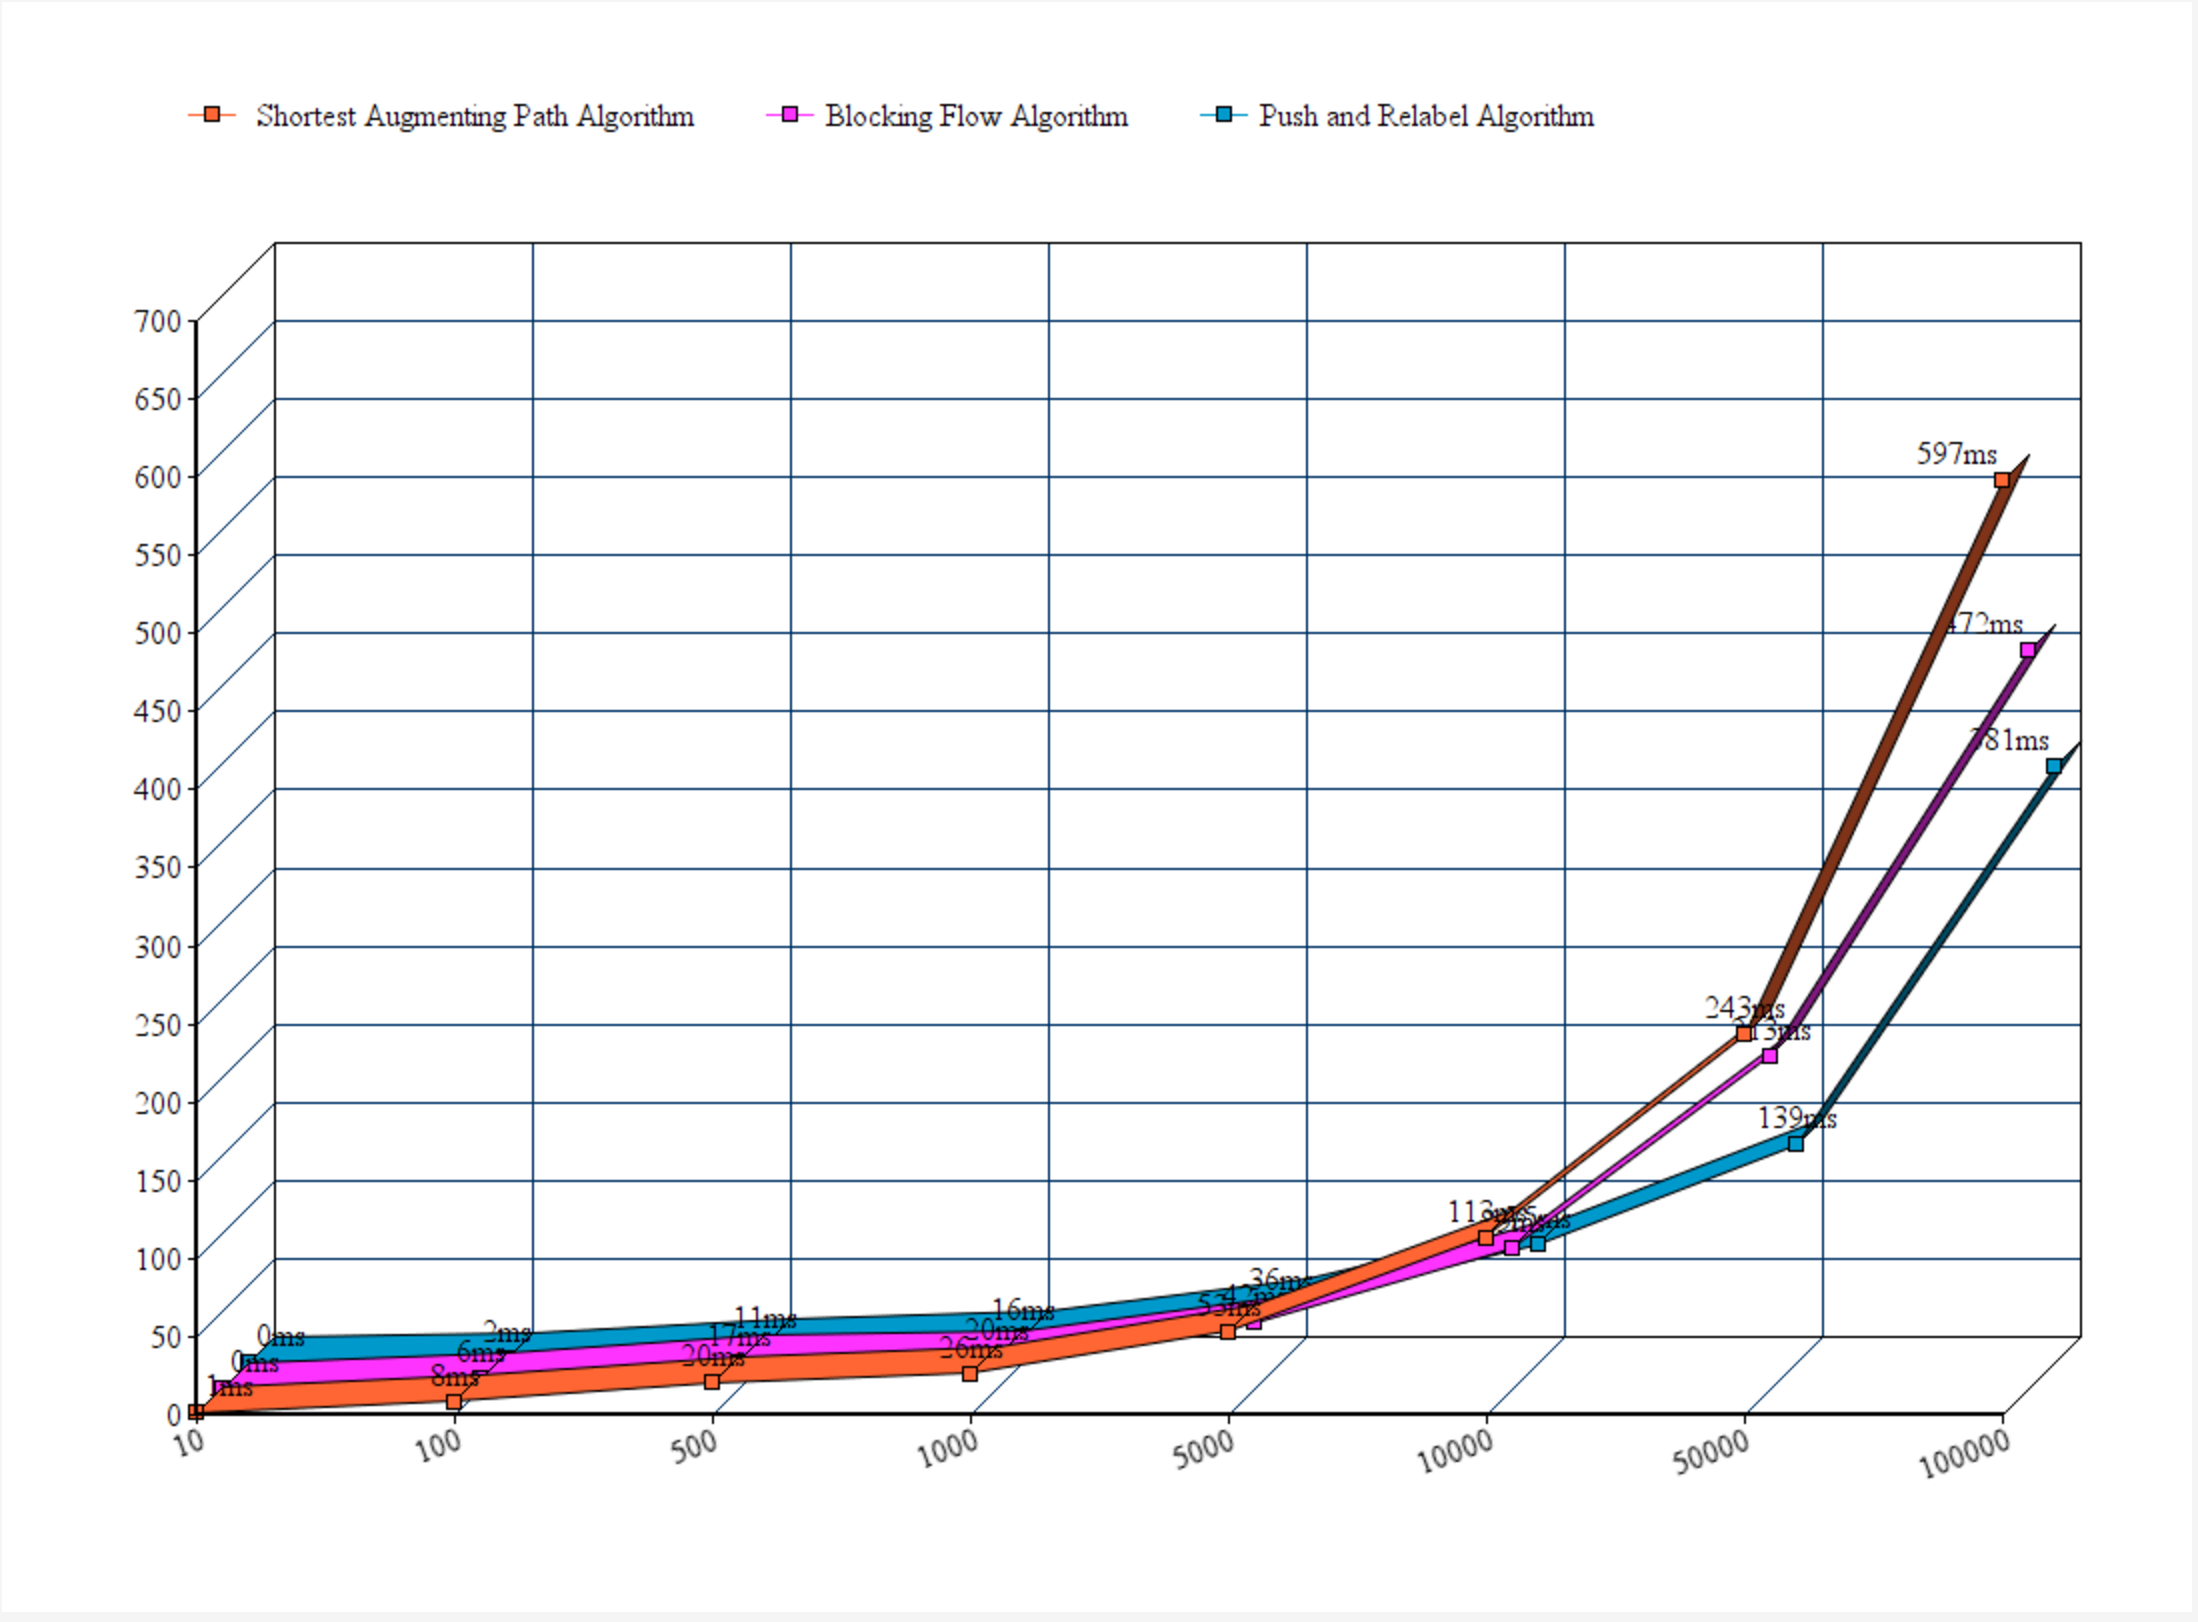
\includegraphics[scale=0.22]{test}


\begin{thebibliography}{1}
	\bibitem{1} L. R. Ford and D. R. Fulkerson. Maximum flow through a network. {\em Can. J. Math. 8}, pages 399-404, 1956.
	\bibitem{2} E. A. Dinic. Algorithm for solution of a problem of maximum flow in networks with power estimation. {\em Soviet Math. Dokl.}, 11:1277-1280, 1970.
	\bibitem{3} J. Edmonds and R. M. Karp. Theoretical improvements in algorithmic efficiency for network flow problems. {\em J. ACM}, 19(2):248-264, April 1972.
	\bibitem{4} R. Tarjan. Depth-first search and linear graph algorithms. {\em SIAM Journal on Computing}, 1(2):146-160, 1972.
	\bibitem{5} A. V. Karzanov. Determining a maximal flow in a network by the method of pre-flows. {\em Soviet Math. Dokl.}, 15(2), 1974.
	\bibitem{6} V. M. Malhotra, M. P. Kumar, and S. N. Maheshwari. An $O(|V|^3)$ algorithm for finding maximum flows in netowkrs. {\em Znf Process. Lett. 7}, pages 277-278, 1978.
	\bibitem{7} Z. Galil. An $O(V^{\frac{5}{3}}E^{\frac{2}{3}})$ algorithm for the maximal flow problem. {\em Acta Inf 2}, pages 221-242, 1980.
	\bibitem{8} D. D. Sleator and R. E. Tarjan. A data structure for dynamic trees. {\em J. Computer and System Science}, 24:362-391, 1983.
	\bibitem{9} R. E. Tarjan. A simple version of karzanov's blocking flow algorithm. {\em Operations Research Letters}, 2(6):265-268, 1984.
	\bibitem{10} H. N. Gabow. Scaling algorithm for network problems. {\em J. Comput. Syst. Sci.}, 31(2):148-168, September 1985.
	\bibitem{11} A. V. Goldberg and R. E. Tarjan. A new approach to the maximum-flow problem. {\em J. ACM}, 35(4):921-940, October 1988.
	\bibitem{12} A. V. Goldberg and R. E. Tarjan. Finding minimum-cost circulations by successive approximation. {\em Mathematics of Operations Research}, 15(3):pp. 430-466, 1990.
	\bibitem{13} N. Alon. Generating pseudo-random permutations and maximum flow algorithms. {\em Inf. Process. Lett., 35(4):201-204}, August 1990.
	\bibitem{14} V. King and S. Rao. A faster deterministic maximum flow algorithm. In {\em Proceedings of the Third Annual ACM-SIAM Symposium on Discrete Algorithms}, SODA '92, pages 157-164, Phiadelphia, PA, USA, 1992. Society for Industrial and Applied Mathematics.
	\bibitem{15} A. V. Goldbery and S. Rao. Beyond the flow decomposition barrier. {\em J. ACM}, 45(5):783-797, September 1998.
	\bibitem{16} Bernhard Haeupler and Robert Endre Tarjan. Finding a feasible flow in a strongly connected network. {\em CoRR}, abs/0711.2710, 2007.
	\bibitem{17} J. B. Orlin. Max flows in $O(nm)$ time, or better. In {\em Proceedings of the Fortyfifth Annual ACM Symposium on Symposium on theory of computing}, SOTC '13, pages 765-774, New York, NY, USA, 2013. ACM.
	\bibitem{18} Computer Vision Research Group at the University of Western Ontario. Max-flow problem instances in vision, http://vision.csd.uwo.ca/maxflow-data, December 2012.
	\bibitem{19} Jakob Mark Friis and Steffen Beier Olesen. An experimental comparison of max flow algorithm. http://www.cs.au.dk/~gerth/advising/thesis/
	


\end{thebibliography}

\end{document}